\documentclass[11pt]{article}
\usepackage[margin=1in]{geometry}
\usepackage{graphicx,amsmath,amssymb,booktabs}
\title{Relation yield per linear system for linearized root finding\\(binary-curve index calculus)}
\author{Isogeny Labs}
\date{25 November 2026\\Interpretation corrected; measurements unchanged}
\begin{document}
\maketitle

\section*{Question}
The linearized root-finding (LRF) kernel made the point-\emph{decomposition} step fast. For index
calculus end to end the step speed is no longer the bottleneck; the \textbf{relation yield per linear
system} is. We measure it, locate where it is lost, and test the two pinned levers: (a) factor bases /
summand counts that raise relations per linear system; (b) the Koblitz / Frobenius structure at prime
$n$. All quantities are counts, measured in exact arithmetic at small prime $n$ where the LRF
decomposition set is cross-checked against enumeration (0 mismatches on every row).

\section*{The funnel}
For $m=3$ and $V=\langle 1,w,\dots,w^{k-1}\rangle$, LRF scans each abscissa $x_3\in V$ and solves one
$\mathbb F_2$-linear system. The funnel is
\[
\text{targets (systems)} \to \text{lin\_solvable} \to \text{lin\_candidates} \to \text{found (relations)},
\]
and $\text{yield/system} = \text{solvable\_rate}\times\text{cand\_per\_solvable}\times\text{found\_per\_cand}$.
The determinacy knob is $\delta = k+\dim V_2-n$; for monomial $V$, $\dim V_2 = 2k-1$, so $\delta=3k-1-n$
and the system is square at $\delta=0$.

\begin{center}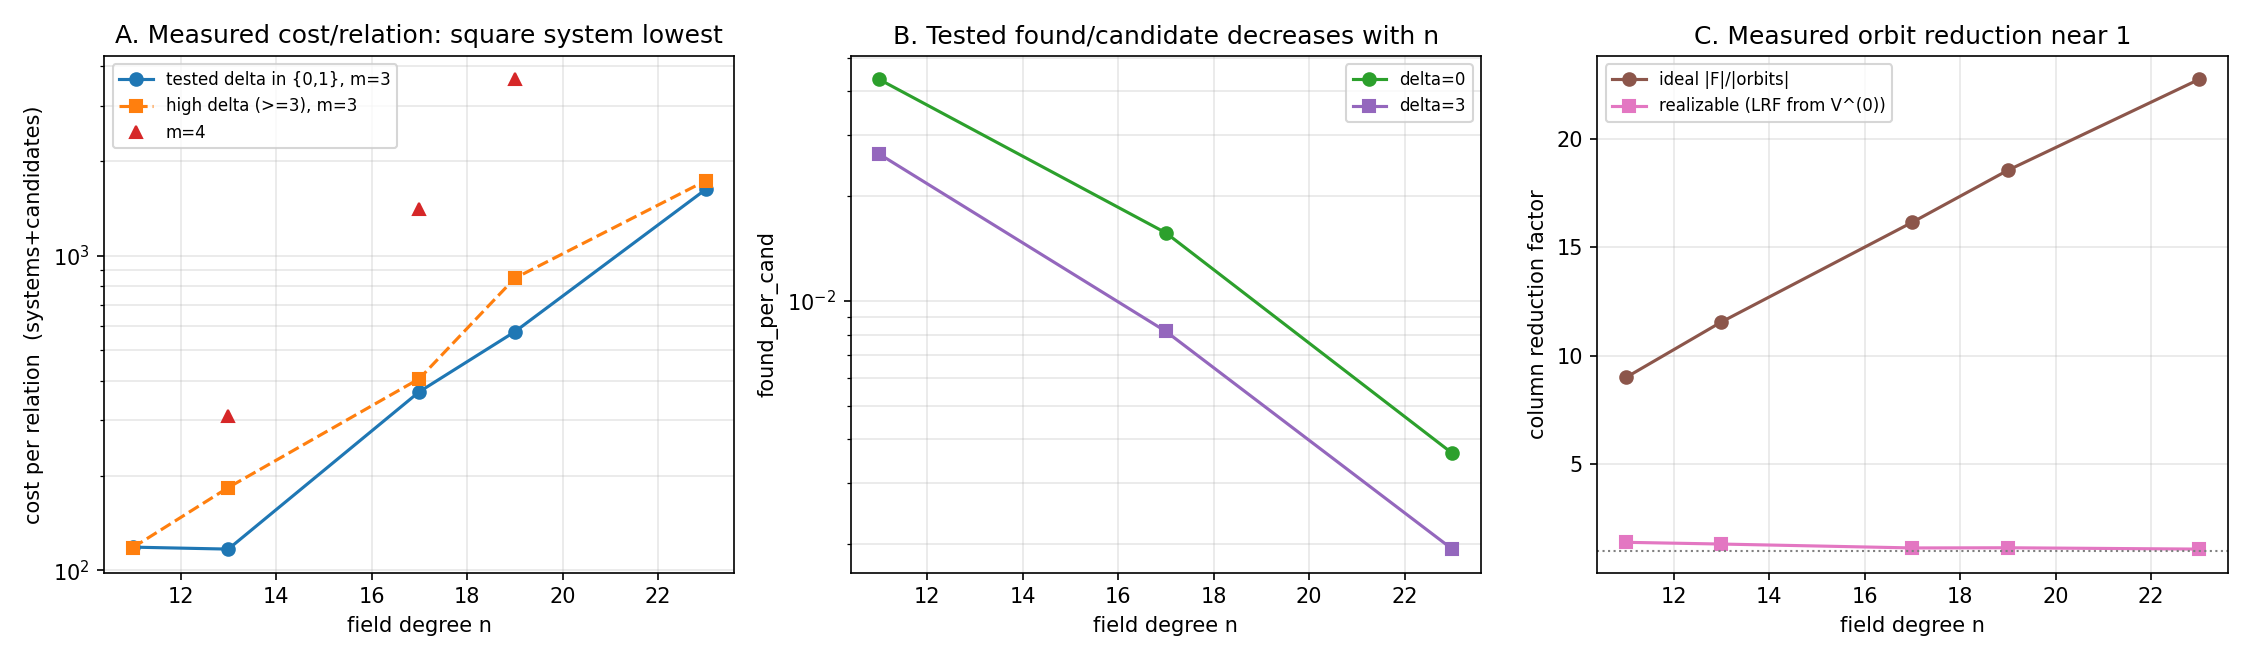
\includegraphics[width=\textwidth]{yield_report.png}\end{center}

\section*{Findings}
\begin{enumerate}
\item \textbf{A square system has the lowest measured cost per relation} ($\delta\in\{0,1\}$,
$m=3$) on this panel (Panel A). High $\delta$ raises yield \emph{per system}, but candidate processing
and factor-base size dominate the measured cost. In the matched cells tested, $m=4$ costs more
than $m=3$.
\item \textbf{Root membership limits measured yield} (Panel B). The chance that both roots of a
candidate quadratic land in $V$ falls across the tested $n$ values at fixed $\delta$. The tested
monomial, $w^2$-power, and shifted bases occupy a similar band. Fixing only $e_1\in V$ and
$e_2\in\mathrm{span}(V\!\cdot\!V)$ does not force the roots into $V$. The measured cost-per-relation
fit is approximately $2^{n/3}$ on this range; it is not a universal lower bound.
\item \textbf{The tested Frobenius construction gives little column reduction} (Panel C).
The $n$ squaring-conjugates $V^{(i)}$ of a monomial $V$ have equal $\dim V_2$, but a search over
one subspace touches almost distinct Frobenius orbits in the tested cells. Measured realizable
column-reduction factors are $1.40,1.32,1.14,1.15,1.09$ for $n=11,\dots,23$.
The tested sliding-window bases share orbits but their product spaces saturate the field at
the sampled dimensions, making this LRF construction infeasible there. Other Frobenius-stable
sets are outside the measurement.
\end{enumerate}

\section*{Consequence for ECC2K-130 ($n=131$) and gap to rho}
For $m=3$, the simple yield model places a monomial base near $k\approx44$ at $n=131$, close to
$\delta=0$. This is a projection from smaller fields, not a measured $n=131$ optimum. The matched
Pollard-rho reference is about $2^{61}$ group operations; a full setup-charged relation-collection
comparison remains required.

\paragraph{Projected ANF degree is not a search lower bound.}
The Boolean success indicator over the kernel coordinates has ANF degree near $\delta$ and density
near $2^{-\delta}$ on the tested systems. This describes the projected
function, not the cost of solving an auxiliary-variable system. For example, the indicator of the
unique point $g=0$ is
\[
\prod_{i=1}^{\delta}(1+g_i),
\]
of degree $\delta$, while $g_i=0$ are linear
defining equations. An exact quadratic root-coordinate lift is documented in the
accompanying screen. Its input degree does not
establish a low solving degree or a cost win; those remain open measurements.
\end{document}
